\subsection[Protótipos]{Protótipos}
Para facilitar a visão de como será o produto de software, a equipe desenvolveu alguns protótipos. Os protótipos permitem que os stakeholders interajam com o produto, assim eles podem ter uma noção de o produto será, e como utilizar o produto [\textbf{X}]. 

A maioria das funcionalidades necessita que o usuário esteja logado. A imagem abaixo mostra o protótipo da tela de login: 

\begin{figure}[!h]
\centering

\includegraphics[scale=0.40, angle = 360]{figuras/prototipo1}
\caption[]{Tela de Login da Aplicação Web (fonte: Autor)}
\end{figure}
\FloatBarrier

Após ter realizado o login, o bibliotecário consegue visualizar um menu com as opções disponíveis. A imagem abaixo apresenta esse menu:

\begin{figure}[!h]
\centering
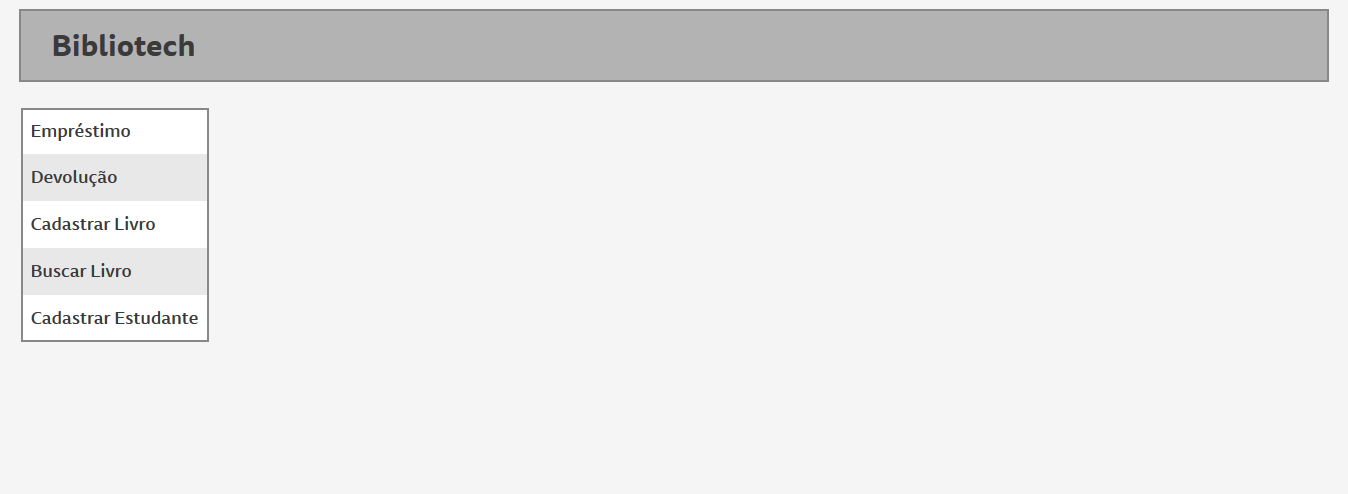
\includegraphics[scale=0.40, angle = 360]{figuras/prototipo2}
\caption[]{Tela inicial do bibliotecário (fonte: Autor)}
\end{figure}
\FloatBarrier

Dado o contexto de uma biblioteca, é interessante que seja realizado o cadastro de estudantes no sistema. Assim, o nosso sistema deve permitir que o bibliotecário cadastre esses alunos. A imagem abaixo mostra o protótipo do cadastro de estudantes:

\begin{figure}[!h]
\centering
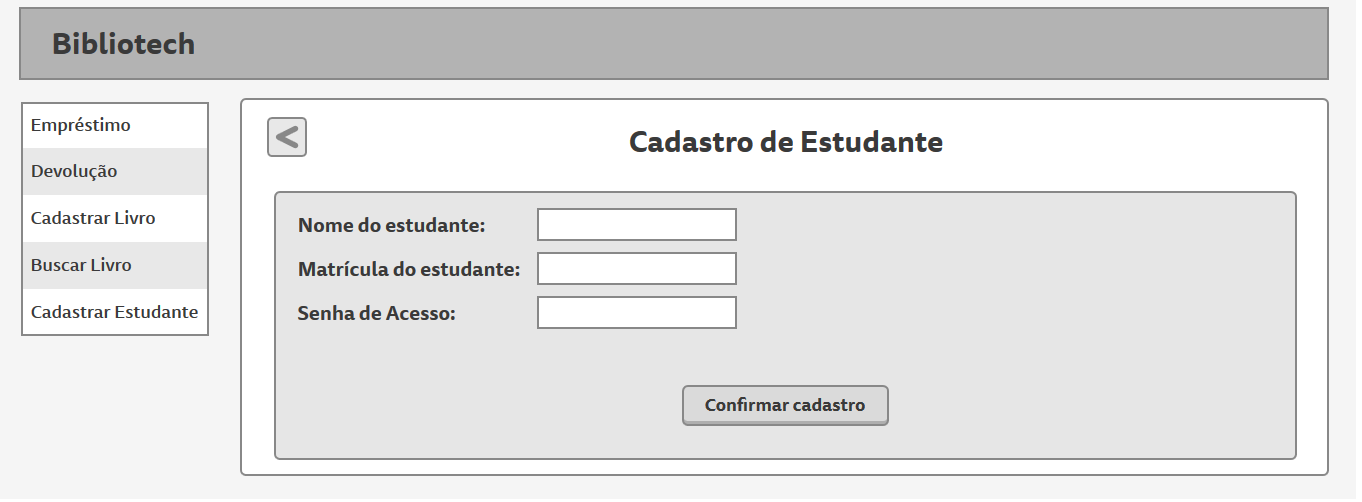
\includegraphics[scale=0.40, angle = 360]{figuras/prototipo3}
\caption[]{Tela de Cadastro de estudantes (fonte: Autor)}
\end{figure}
\FloatBarrier

Também é interessante permitir ao bibliotecário o cadastro de livros e a edição de livros. No momento do cadastro, o sistema verifica uma posição disponível e aloca esse livro a uma posição. A imagem abaixo apresenta as telas do cadastro/edição de livros:

\begin{figure}[!h]
\centering
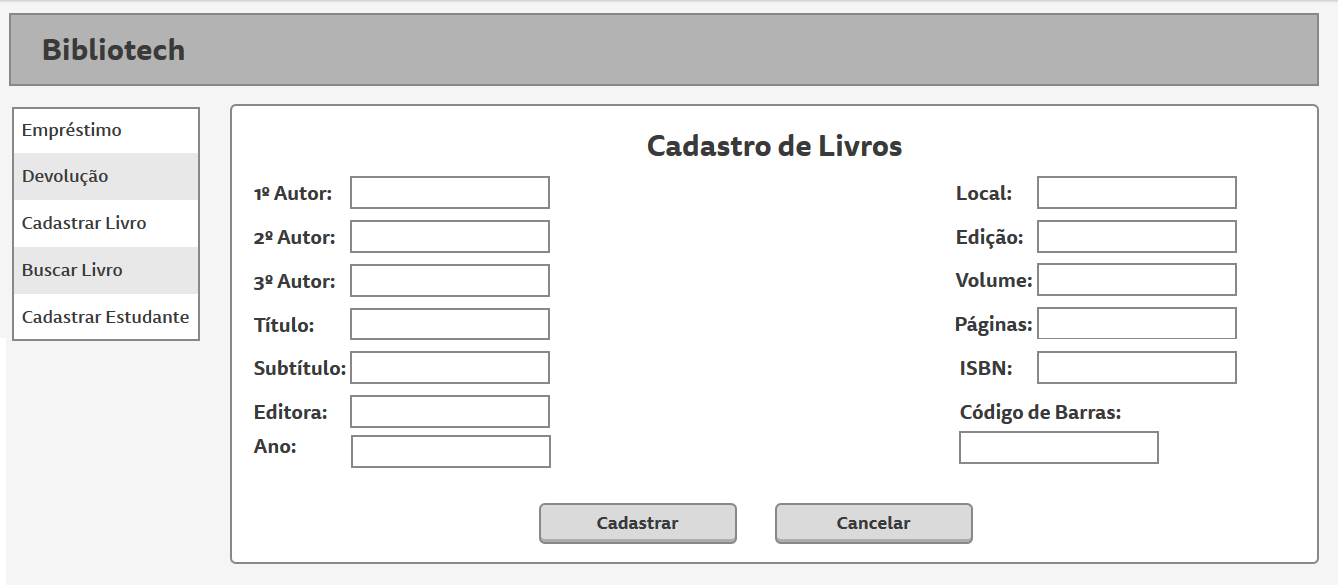
\includegraphics[scale=0.40, angle = 360]{figuras/prototipo4}
\caption[]{Tela de cadastro/edição de livros (fonte: Autor)}
\end{figure}
\FloatBarrier

O sistema deverá permitir que tanto o estudante quanto o bibliotecário pesquisem livros, para realizarem eventuais consultas. A imagem abaixo mostra a tela de pesquisa:

\begin{figure}[!h]
\centering
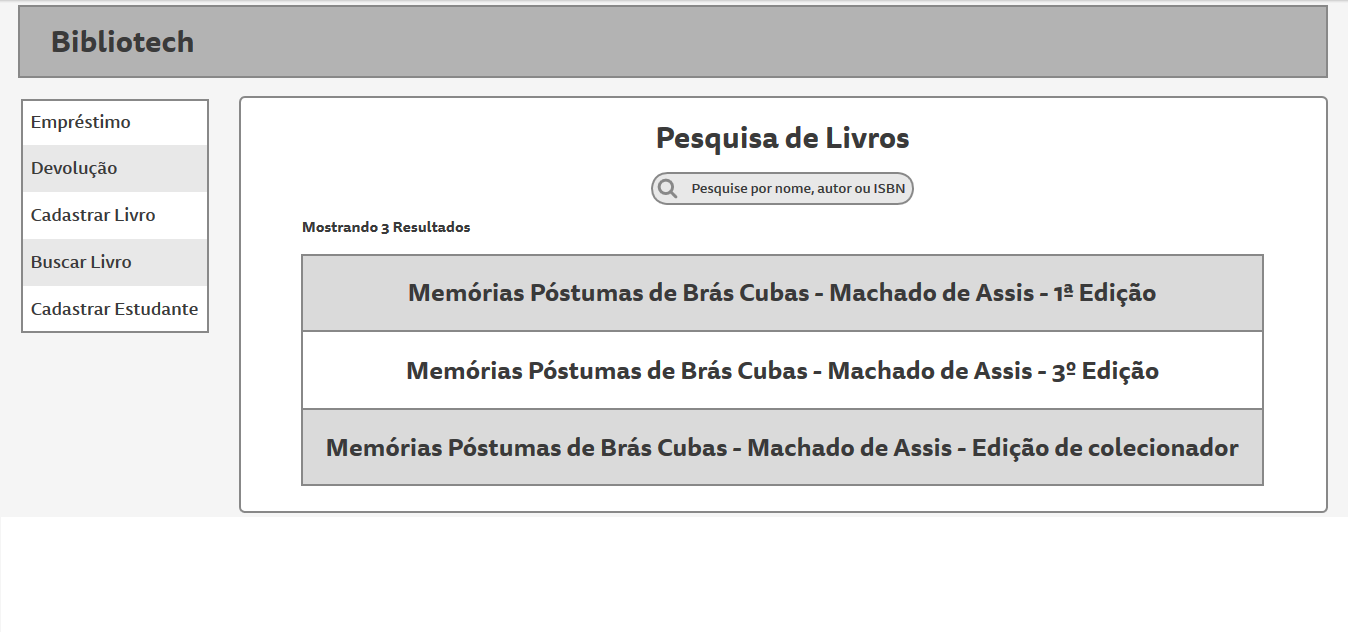
\includegraphics[scale=0.40, angle = 360]{figuras/prototipo5}
\caption[]{Tela de pesquisa de livros (fonte: Autor)}
\end{figure}
\FloatBarrier

Após a pesquisa, o estudante ou o bibliotecário irá escolher um dos livros e realizar a consulta. Para o estudante, é informado o status do livro e uma mensagem. Caso o livro não esteja disponível, é mostrada o opção de  agendar livro. A imagem abaixo e a imagem subsequente mostra a tela de consulta do estudante e a imagem \textbf{X}, mostra a tela de agendamento:

\begin{figure}[!h]
\centering
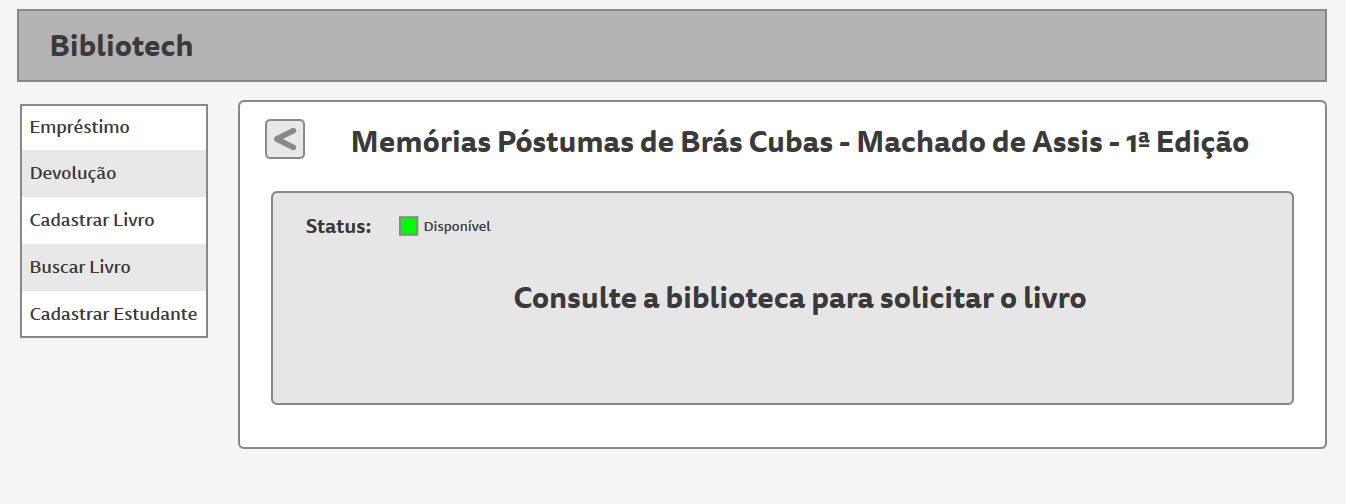
\includegraphics[scale=0.40, angle = 360]{figuras/prototipo6}
\caption[]{Tela de consulta de livro do estudante (fonte: Autor)}
\end{figure}
\FloatBarrier

\begin{figure}[!h]
\centering
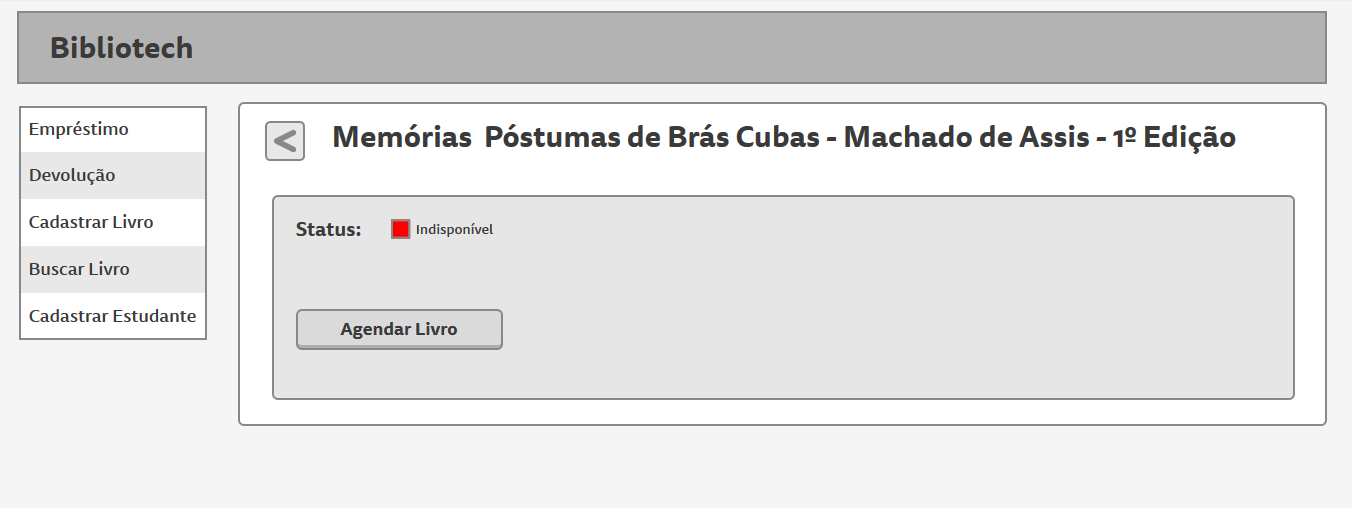
\includegraphics[scale=0.40, angle = 360]{figuras/prototipo7}
\caption[]{Tela de consulta de livro do estudante (fonte: Autor)}
\end{figure}
\FloatBarrier

\begin{figure}[!h]
\centering
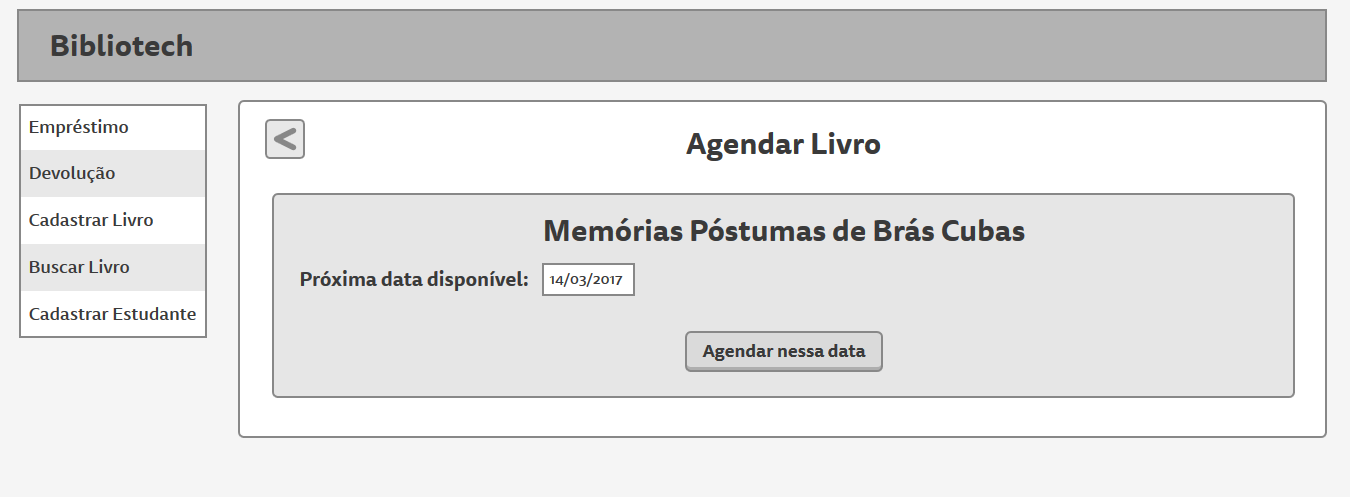
\includegraphics[scale=0.40, angle = 360]{figuras/prototipo8}
\caption[]{Tela de consulta de livro do estudante (fonte: Autor)}
\end{figure}
\FloatBarrier

Na consulta, para o bibliotecário, é informado o estado do livro e um botão para iniciar o empréstimo. A imagem \textbf{X} mostra a tela de consulta do bibliotecário:

\begin{figure}[!h]
\centering
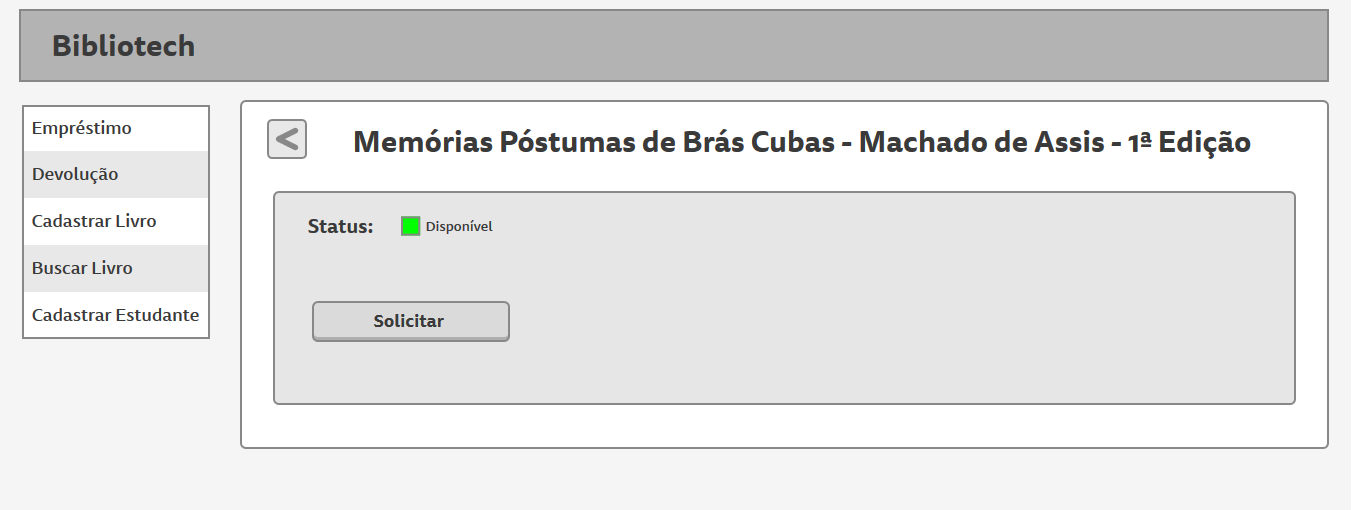
\includegraphics[scale=0.40, angle = 360]{figuras/prototipo9}
\caption[]{Tela de consulta livro bibliotecário (fonte: Autor)}
\end{figure}
\FloatBarrier

Após a solicitação do livro, o robô trará o livro para o bibliotecário e ele inserirá as informações do estudante, confirmando o empréstimo. A imagem abaixo mostra a tela de empréstimo:

\begin{figure}[!h]
\centering
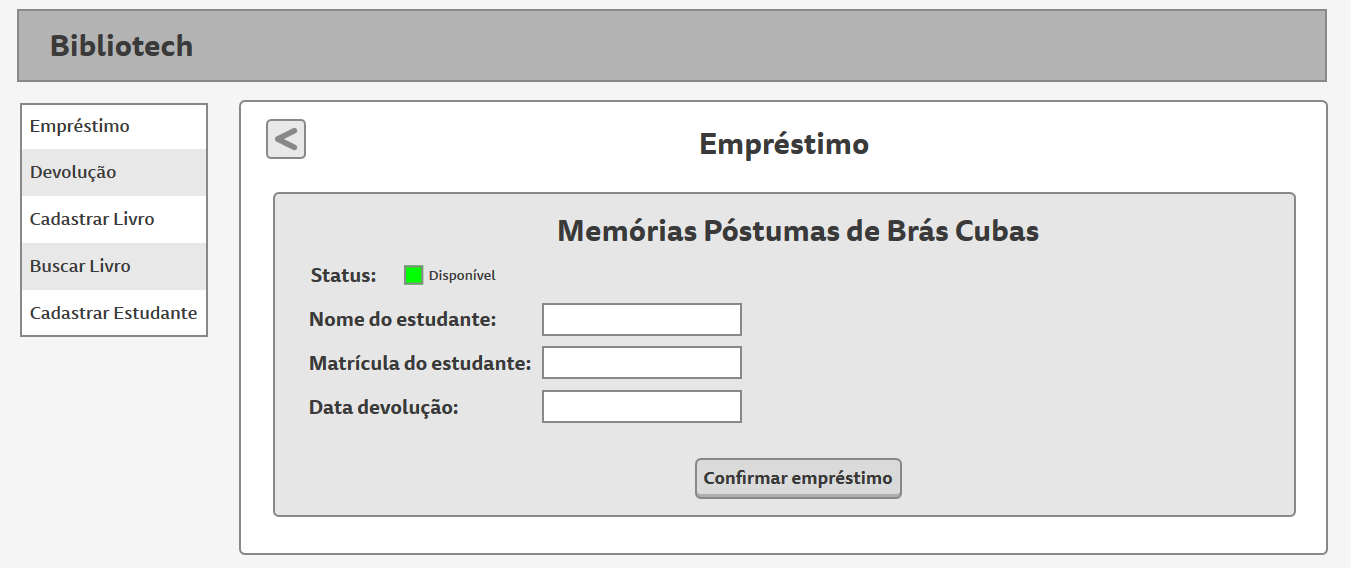
\includegraphics[scale=0.40, angle = 360]{figuras/prototipo10}
\caption[]{Tela de empréstimo de livros (fonte: Autor)}
\end{figure}
\FloatBarrier

Quando o aluno for devolver o livro, o bibliotecário irá inserir o código de barras do livro, o sistema carregará as informações relativas ao livro, e o bibliotecário escolherá a opção de confirmar a devolução. A imagem abaixo apresenta a tela de devolução do livro:

\begin{figure}[!h]
\centering
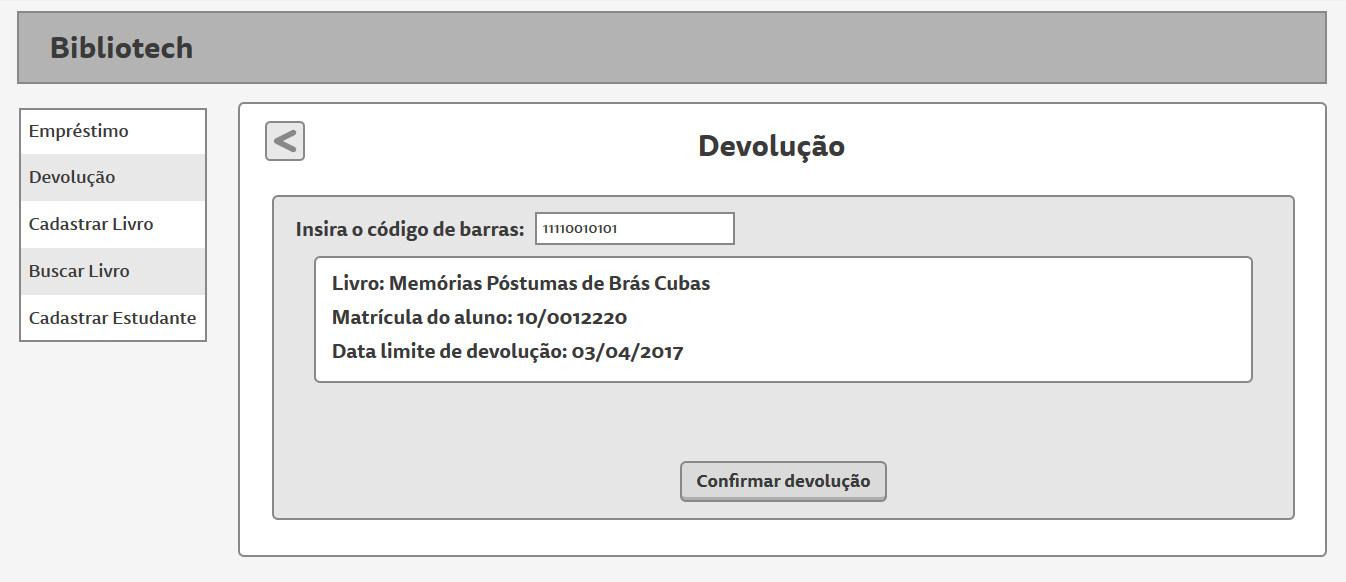
\includegraphics[scale=0.40, angle = 360]{figuras/prototipo11}
\caption[]{Tela de devolução de livros (fonte: Autor)}
\end{figure}
\FloatBarrier